\documentclass[a4paper, 11pt]{article}
\usepackage[utf8]{inputenc}
\usepackage[T1]{fontenc}
\usepackage[margin = 20mm, head = 10mm, foot = 0mm]{geometry}
\usepackage{graphicx, longtable, wrapfig, amsmath, textcomp, amssymb, hyperref}
\usepackage{fancyhdr, lastpage, marvosym, titlesec, tabularx}

\hypersetup{
  colorlinks = true,
  urlcolor   = blue,
  pdfauthor  = {Marek Felšöci},
  pdftitle   = {Curriculum Vitae},
  pdflang    = {English}
}

\setlength{\parskip}{2mm}
\setlength{\parindent}{0pt}

\renewcommand{\headrulewidth}{0pt}
\titleformat{\section}{\normalfont\large\bfseries}{\thesection}{1em}{}
            [{\titlerule[0.8pt]}]

\pagestyle{fancy}
\fancyhf{}
\rfoot{\thepage/\pageref{LastPage}}

\title{Curriculum Vitae}
\date{}

\begin{document}

\begin{center}
  {\Huge\bfseries\scshape Marek Felšöci} \\ [2mm]
  12 Rue Fonfrède | 33800 Bordeaux | France \\ [1mm]
  \Telefon\ +33 5 33 05 12 61 | \Mobilefone\ +33 7 81 17 58 79  \\ [1mm]
  \Letter\ \href{mailto:marek@felsoci.sk}{marek@felsoci.sk} |
  \Info\ \href{https://www.felsoci.sk}{https://www.felsoci.sk}
\end{center}

\section*{EDUCATION}

\begin{tabularx}{\linewidth}{cXr}
  2019 - \phantom{2023} & \textbf{Inria Bordeaux Sud-Ouest} &
    \emph{Bordeaux, France} \\
  & \multicolumn{2}{
      >{\hsize = \dimexpr2\hsize+2\tabcolsep+\arrayrulewidth\relax}X
    }{\textsc{Ph.D. thesis: Fast solvers for high-frequency aeroacoustics}} \\
  & \textit{HiePACS team} & \\
  & \multicolumn{2}{
      >{\hsize = \dimexpr2\hsize+2\tabcolsep+\arrayrulewidth\relax}X
    }{\textit{supervised by Guillaume Sylvand and Emmanuel Agullo}} \\
  & \multicolumn{2}{
      >{\hsize = \dimexpr2\hsize+2\tabcolsep+\arrayrulewidth\relax}X
    }{
      Developing efficient methods for solving large coupled sparse/dense
      FEM/BEM linear systems arising from aeroacoustic problems in the
      industrial context of Airbus
    } \\
\end{tabularx}

\begin{tabularx}{\linewidth}{cXr}
  2017 - 2019 & \textbf{University of Strasbourg} & \emph{Strasbourg, France} \\
  & \multicolumn{2}{
      >{\hsize = \dimexpr2\hsize+2\tabcolsep+\arrayrulewidth\relax}X
    }{\textsc{Master's degree in Computer Science}} \\
  & \textit{with honors (mention bien)} & \\
  & \multicolumn{2}{
      >{\hsize = \dimexpr2\hsize+2\tabcolsep+\arrayrulewidth\relax}X
    }{
      Compilation and code optimization, Parallel computing, Distributed systems
      and grids, Embedded and real-time systems, Electronics, Performance
      evaluation, Networking protocols, Routing, Security, Internet of Things
    } \\
\end{tabularx}

\begin{tabularx}{\linewidth}{cXr}  
  2014 - 2017 & \textbf{University of Strasbourg} & \emph{Strasbourg, France} \\
  & \multicolumn{2}{
      >{\hsize = \dimexpr2\hsize+2\tabcolsep+\arrayrulewidth\relax}X
    }{\textsc{Bachelor's degree in Computer Science}} \\
  & \textit{with honors (mention assez bien)} & \\
  & \multicolumn{2}{
      >{\hsize = \dimexpr2\hsize+2\tabcolsep+\arrayrulewidth\relax}X
    }{
      Programming, Data structures and algorithms, Language theory, Logic, Graph
      theory, Operating systems, Web development, Database management
    } \\
\end{tabularx}

\begin{tabularx}{\linewidth}{cXr}
  2012 - 2014 & \textbf{Lycée Pilote Innovant International} &
    \emph{Jaunay-Clan, France} \\
  & \multicolumn{2}{
      >{\hsize = \dimexpr2\hsize+2\tabcolsep+\arrayrulewidth\relax}X
    }{\textsc{International High School}} \\
  & \textit{with honors (mention assez bien)} & \\
  & \multicolumn{2}{
      >{\hsize = \dimexpr2\hsize+2\tabcolsep+\arrayrulewidth\relax}X
    }{Scientific section with emphasis on mathematics} \\
\end{tabularx}

\begin{tabularx}{\linewidth}{cXr}
  2011 - 2013 & \textbf{Gymnázium M. R. Štefánika} &
    \emph{Košice, Slovakia} \\
  & \multicolumn{2}{
      >{\hsize = \dimexpr2\hsize+2\tabcolsep+\arrayrulewidth\relax}X
    }{\textsc{Bilingual French-Slovak High School}} \\
  & \multicolumn{2}{
      >{\hsize = \dimexpr2\hsize+2\tabcolsep+\arrayrulewidth\relax}X
    }{
      Proposal to attend Lycée Pilote Innovant International after the first
      year
    } \\
\end{tabularx}

\section*{RESEARCH INTERESTS}

solution of large linear systems, high-performance computing, compiler design,
code optimization

\section*{INTERNSHIPS}

\begin{tabularx}{\linewidth}{cXr}
  01 - 07/2019 & \textbf{ICube} & \emph{Strasbourg, France} \\
  & \multicolumn{2}{
      >{\hsize = \dimexpr2\hsize+2\tabcolsep+\arrayrulewidth\relax}X
    }{\textsc{Research Intern}} \\
  & \textit{Scientific and Parallel Computing team} & \\
  & \multicolumn{2}{
      >{\hsize = \dimexpr2\hsize+2\tabcolsep+\arrayrulewidth\relax}X
    }{\textit{Supervised by Philippe Clauss}} \\
  & \multicolumn{2}{
      >{\hsize = \dimexpr2\hsize+2\tabcolsep+\arrayrulewidth\relax}X
    }{
      Integration of the XFOR programming structure into the Clang/LLVM
      compiler and extension to parallel programming
    } \\
\end{tabularx}

\begin{tabularx}{\linewidth}{cXr}
  05 - 08/2018 & \textbf{ICube} & \emph{Strasbourg, France} \\
  & \multicolumn{2}{
      >{\hsize = \dimexpr2\hsize+2\tabcolsep+\arrayrulewidth\relax}X
    }{\textsc{Research Intern}} \\
  & \textit{Scientific and Parallel Computing team} & \\
  & \multicolumn{2}{
      >{\hsize = \dimexpr2\hsize+2\tabcolsep+\arrayrulewidth\relax}X
    }{\textit{Supervised by Philippe Clauss}} \\
  & \multicolumn{2}{
      >{\hsize = \dimexpr2\hsize+2\tabcolsep+\arrayrulewidth\relax}X
    }{Extension of the XFOR structure programming tools} \\
\end{tabularx}

\begin{tabularx}{\linewidth}{cXr}
  05 - 08/2017 & \textbf{Mageek} & \emph{Strasbourg, France} \\
  & \multicolumn{2}{
      >{\hsize = \dimexpr2\hsize+2\tabcolsep+\arrayrulewidth\relax}X
    }{\textsc{Development Intern}} \\
  & \multicolumn{2}{
      >{\hsize = \dimexpr2\hsize+2\tabcolsep+\arrayrulewidth\relax}X
    }{\textit{Supervised by Stéphane Heitz}} \\
  & \multicolumn{2}{
      >{\hsize = \dimexpr2\hsize+2\tabcolsep+\arrayrulewidth\relax}X
    }{Development of a content management system} \\
\end{tabularx}

\begin{tabularx}{\linewidth}{cXr}
  05 - 08/2017 & \textbf{United States Steel Košice} &
    \emph{Košice, Slovakia} \\
  & \multicolumn{2}{
      >{\hsize = \dimexpr2\hsize+2\tabcolsep+\arrayrulewidth\relax}X
    }{\textsc{Development Intern}} \\
  & \multicolumn{2}{
      >{\hsize = \dimexpr2\hsize+2\tabcolsep+\arrayrulewidth\relax}X
    }{\textit{Supervised by Martina Koperová}} \\
  & \multicolumn{2}{
      >{\hsize = \dimexpr2\hsize+2\tabcolsep+\arrayrulewidth\relax}X
    }{Internal website development and intranet maintenance} \\
\end{tabularx}

\subsection*{Publications}
\label{sec:orgd6422e8}
Items below are sorted by date of publication from the most to the least recent.
Author names always appear in alphabetical order.

\begin{itemize}
\item \textbf{Numerical Modelisation of Interaction between Plasma Thruster Plume and}
\textbf{Antennas on Small Satellites}
\begin{itemize}
\item T. Abboud, B. Chaigne, \emph{M. Felšöci}, A. Piche and G. Sylvand
\item \href{https://waves2022.apps.math.cnrs.fr/}{Waves 2022} - International
Conference on Mathematical and Numerical Aspects of Wave Propagation, 2022
\end{itemize}
\item \textbf{Direct solution of larger coupled sparse/dense linear systems using low-rank}
\textbf{compression on single-node multi-core machines in an industrial context}
\begin{itemize}
\item E. Agullo, \emph{M. Felšöci} and G. Sylvand
\item \href{http://www.ipdps.org/ipdps2022/index.html}{IPDPS 2022} - IEEE
International Parallel and Distributed Processing Symposium, 2022,
pp. 25–35
\item \begin{center}
%
\includegraphics[width=.9\linewidth]{./images/html.png}
\end{center}
\href{https://doi.ieeecomputersociety.org/10.1109/IPDPS53621.2022.00012}{Article}
\item \begin{center}
%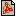
\includegraphics[width=.9\linewidth]{./images/pdf.png}
\end{center}
\href{https://thesis-mfelsoci.gitlabpages.inria.fr/thesis/slides/ipdps-2022.pdf}{Slides}
\item \begin{center}
%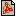
\includegraphics[width=.9\linewidth]{./images/pdf.png}
\end{center} \href{https://hal.inria.fr/hal-03557692/document}{Research
report}
\end{itemize}
\item \textbf{Guix-HPC Activity Report 2020-2021}
\begin{itemize}
\item P.-A. Bouttier, L. Courtès, Y. Dupont, \emph{M. Felšöci}, F. Gruber, K. Hinsen,
A. Isaac, P. Prins, P. Swartvagher, S. Tournier and R. Wurmus
\item Inria Bordeaux - Sud-Ouest, Université Grenoble - Alpes, Université Paris,
Technical Report, 2022
\item \begin{center}
%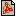
\includegraphics[width=.9\linewidth]{./images/pdf.png}
\end{center} \href{https://hal.inria.fr/hal-03565692/document}{Technical
report}
\end{itemize}
\item \textbf{Study of the processor and memory power consumption of coupled sparse/dense}
\textbf{solvers}
\begin{itemize}
\item E. Agullo, \emph{M. Felšöci}, A. Guermouche, H. Mathieu, G. Sylvand and B.
Tagliaro
\item Inria Bordeaux Sud-Ouest, Research Report RR-9463, 2022
\item \begin{center}
%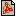
\includegraphics[width=.9\linewidth]{./images/pdf.png}
\end{center} \href{https://hal.inria.fr/hal-03589695/document}{Research
report}
\end{itemize}
\item \textbf{Comparison of coupled solvers for FEM/BEM linear systems arising from}
\textbf{discretization of aeroacoustic problems}
\begin{itemize}
\item E. Agullo, \emph{M. Felšöci} and G. Sylvand
\item \href{https://2021.compas-conference.fr/}{COMPAS 2021} - Conférence francophone
d’informatique en Parallélisme, Architecture et Système, 2021
\item \begin{center}
%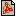
\includegraphics[width=.9\linewidth]{./images/pdf.png}
\end{center} \href{https://hal.inria.fr/hal-03264472/document}{Article}
\item \begin{center}
%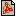
\includegraphics[width=.9\linewidth]{./images/pdf.png}
\end{center} \begin{center}
%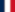
\includegraphics[width=.9\linewidth]{./images/fr.png}
\end{center}
\href{https://thesis-mfelsoci.gitlabpages.inria.fr/thesis/slides/compas-2021.pdf}{Slides}
\end{itemize}
\item \textbf{A comparison of selected solvers for coupled FEM/BEM linear systems arising}
\textbf{from discretization of aeroacoustic problems}
\begin{itemize}
\item E. Agullo, \emph{M. Felšöci} and G. Sylvand
\item Inria Bordeaux Sud-Ouest, Research Report RR-9412, 2021
\item \begin{center}
%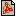
\includegraphics[width=.9\linewidth]{./images/pdf.png}
\end{center} \href{https://hal.inria.fr/hal-03263603/document}{Research
report}
\end{itemize}
\item \textbf{A comparison of selected solvers for coupled FEM/BEM linear systems arising}
\textbf{from discretization of aeroacoustic problems: literate and reproducible}
\textbf{environment}
\begin{itemize}
\item E. Agullo, \emph{M. Felšöci} and G. Sylvand
\item Inria Bordeaux Sud-Ouest, Technical Report RT-0513, 2021
\item \begin{center}
%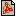
\includegraphics[width=.9\linewidth]{./images/pdf.png}
\end{center} \href{https://hal.inria.fr/hal-03263620/document}{Technical
report}
\end{itemize}
\end{itemize}

\subsection*{Talks}
\label{sec:org5399215}
\begin{itemize}
\item \textbf{Solution of larger coupled sparse/dense linear systems in an industrial}
\textbf{aeroacoustic context}
\begin{itemize}
\item \href{https://team.inria.fr/camus/}{CAMUS team} seminar @ ICube lab,
Illkirch-Graffenstaden, France, June 2022
\item \begin{center}
%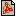
\includegraphics[width=.9\linewidth]{./images/pdf.png}
\end{center}
\href{https://thesis-mfelsoci.gitlabpages.inria.fr/slides/camus/camus.pdf}{Slides}
\end{itemize}
\item \textbf{Guix and Org mode, a powerful association for building a reproducible}
\textbf{research study}
\begin{itemize}
\item Seminar and hands-on session @ Inria Grand-Est, Nancy, France, June 2022
\item \begin{center}
%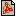
\includegraphics[width=.9\linewidth]{./images/pdf.png}
\end{center}
\href{https://tuto-techno-guix-hpc.gitlabpages.inria.fr/slides/tuto-techno-guix-hpc.pdf}{Slides}
\item \begin{center}
%
\includegraphics[width=.9\linewidth]{./images/html.png}
\end{center}
\href{https://tuto-techno-guix-hpc.gitlabpages.inria.fr/guidelines/}{Hands-on
session}
\end{itemize}
\item \textbf{Direct solution of larger coupled sparse/dense FEM/BEM linear systems using}
\textbf{low-rank compression}
\begin{itemize}
\item \href{https://sparsedays.cerfacs.fr/}{Sparse Days 2022} @ St-Girons, France,
June 2022
\item \begin{center}
%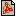
\includegraphics[width=.9\linewidth]{./images/pdf.png}
\end{center}
\href{https://thesis-mfelsoci.gitlabpages.inria.fr/slides/sparse-days/sparse-days.pdf}{Slides}
\end{itemize}
\item \textbf{Reconciling high-performance computing with the use of third-party}
\textbf{libraries?}
\begin{itemize}
\item with E. Agullo
\item \href{https://team.inria.fr/datamove/}{Datamove team} seminar, held virtually,
May 2022
\item \begin{center}
%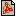
\includegraphics[width=.9\linewidth]{./images/pdf.png}
\end{center}
\href{https://thesis-mfelsoci.gitlabpages.inria.fr/slides/datamove/datamove.pdf}{Slides}
\end{itemize}
\item \textbf{An energy consumption study of coupled solvers for FEM/BEM linear systems:}
\textbf{preliminary results}
\begin{itemize}
\item \href{https://www.irit.fr/solharis/solharis-plenary-meeting-09-10-02-2022/}{SOLHARIS
plenary meeting} @ Inria Bordeaux Sud-Ouest, Bordeaux, France, February
2022
\item \begin{center}
%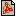
\includegraphics[width=.9\linewidth]{./images/pdf.png}
\end{center}
\href{https://www.irit.fr/solharis/wp-content/uploads/2022/02/022022\_marek\_felsoci.pdf}{Slides}
\end{itemize}
\item \textbf{Towards memory-aware multi-solve two-stage solver for coupled FEM/BEM}
\textbf{systems}
\begin{itemize}
\item \href{https://www.irit.fr/solharis/solharis-plenary-meeting-02-07-2021/}{SOLHARIS
plenary meeting}, held virtually, July 2021
\item \begin{center}
%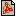
\includegraphics[width=.9\linewidth]{./images/pdf.png}
\end{center}
\href{https://www.irit.fr/solharis/wp-content/uploads/2021/07/072021\_felsoci.pdf}{Slides}
\end{itemize}
\item \textbf{Coupled solvers for high-frequency aeroacoustics}
\begin{itemize}
\item Doctoral school days, held virtually, May 2021
\item \begin{center}
%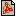
\includegraphics[width=.9\linewidth]{./images/pdf.png}
\end{center}
\href{https://thesis-mfelsoci.gitlabpages.inria.fr/thesis/slides/poster-edmi-days.pdf}{Poster}
\end{itemize}
\item \begin{center}
%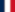
\includegraphics[width=.9\linewidth]{./images/fr.png}
\end{center} \textbf{Guix et Org mode, deux amis du doctorant sur le chemin}
\textbf{vers une thèse reproductible}
\begin{itemize}
\item \href{https://hpc.guix.info/events/2021/atelier-reproductibilit\%C3\%A9-environnements/}{Atelier
reproductibilité des environnements logiciels}, held virtually, May 2021
\item \begin{center}
%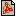
\includegraphics[width=.9\linewidth]{./images/pdf.png}
\end{center}
\href{https://hpc.guix.info/static/doc/atelier-reproductibilit\%C3\%A9-2021/marek-fel\%C5\%A1\%C3\%B6ci-org-guix.pdf}{Slides}
\item \begin{center}
%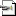
\includegraphics[width=.9\linewidth]{./images/video.png}
\end{center}
\href{https://hpc.guix.info/static/videos/atelier-reproductibilit\%C3\%A9-2021/marek-fel\%C5\%A1\%C3\%B6ci.webm}{Video
recording}
\end{itemize}
\item \textbf{Coupled solvers for FEM/BEM linear systems arising from discretization of}
\textbf{aeroacoustic problems}
\begin{itemize}
\item \href{https://team.inria.fr/hiepacs/}{HiePACS team} work group, held virtually,
April 2021
\item \begin{center}
%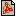
\includegraphics[width=.9\linewidth]{./images/pdf.png}
\end{center}
\href{https://thesis-mfelsoci.gitlabpages.inria.fr/thesis/slides/wg-04-2021.pdf}{Slides}
\end{itemize}
\item \textbf{A preliminary comparative study of solvers for coupled FEM/BEM linear}
\textbf{systems in a reproducible environment}
\begin{itemize}
\item \href{https://www.irit.fr/solharis/solharis-plenary-meeting-07-08-12-2020/}{SOLHARIS
plenary meeting}, held virtually, December 2020
\item \begin{center}
%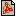
\includegraphics[width=.9\linewidth]{./images/pdf.png}
\end{center}
\href{https://www.irit.fr/solharis/wp-content/uploads/2020/12/122020-Felsoci.pdf}{Slides}
\end{itemize}
\end{itemize}

\section*{Projects}
\label{sec:org1ac0fff}

\textbf{Parallel computational kernels for matrix multiplication}

\textsc{University project}, \emph{2 members}

Implemented multiple parallel computational kernels for matrix multiplication
using the nVidia CUDA technology.

\vspace{1em}

\textbf{Parallelization strategy for labyrinth generation}

\textsc{University project}, \emph{individual}

Proposed and implemented a parallelization strategy for labyrinth generation
process using the MPI technology.

\vspace{1em}

\textbf{StenC language compiler}

\textsc{University project}, \emph{2 members}

Developed a simple DSL compiler from scratch which allows to easily apply
stencils to images.

\vspace{1em}

\textbf{Embedded Snake game}

\textsc{University project}, \emph{4 members}

Developed and deployed a joystick controlled version of Snake on the Texas
Instruments MSP432 board.

\vspace{1em}

\textbf{Embedded video player}

\textsc{University project}, \emph{2 members}

Configured, cross-compiled and deployed Linux kernel together with a video
player on the Texas Instruments OMAP-L138 board.

\vspace{1em}

\textbf{Backy}

\textsc{Personal project}, \emph{individual}

Developed an intuitive, straightforward and multi-platform file backup solution
in C++.

\vspace{1em}

\textbf{Slovoca}

\textsc{Personal project}, \emph{individual}

Developed a custom dictionary manager in C\# to help me with learning of foreign
languages.

\section*{Expertise}
\label{sec:org7bbe237}

\begin{itemize}
\item \textbf{Programming:} C, C++, Fortran, C\#, Java, Python, Caml, Elisp, Prolog, MIPS
\item \textbf{Compilation:} LLVM, Clang, Lex and Yacc
\item \textbf{Parallelization:} POSIX and Windows threads, OpenMP, MPI, CUDA
\item \textbf{Polyhedral optimization:} ISL, OpenScop, Polly, ClooG, Clan, Candl
\item \textbf{Scripting:} Bash, Batch, PowerShell
\item \textbf{Web development:} JavaScript, react.js, PHP, node.js
\item \textbf{Databases:} PL/SQL, MySQL, MongoDB
\item \textbf{Network administration:} Juniper, Cisco, IPv4 and IPv6
\item \textbf{Miscellaneous:} Unix and Windows systems, GDB, Valgrind, Git, Subversion,
\LaTeX, GNS3, Arduino, Emacs, Org mode
\end{itemize}

\section*{Language skills}
\label{sec:orgdf7fdb1}

\textbf{French} (bilingual), \textbf{English} (fluent), \textbf{Slovak} (mother tongue), \textbf{Czech}
(bilingual), \textbf{Ukra\-ini\-an} (intermediate)

\section*{Free-time activities}
\label{sec:org3c85015}

learning new foreign languages, reading (detective and fantasy novels,
linguistics and history-related books), biking
\end{document}
